%----------------------------------------------------------------------------------------
%	PACKAGES AND THEMES
%----------------------------------------------------------------------------------------
\documentclass[aspectratio=169,xcolor=dvipsnames]{beamer}
\usepackage[english,russian]{babel}
\usetheme{Simple}

\usepackage{hyperref}
\usepackage{graphicx} % Allows including images
\usepackage{booktabs} % Allows the use of \toprule, \midrule and \bottomrule in tables

\usepackage{tikz}
\usetikzlibrary{shapes.geometric, arrows.meta, positioning}

\tikzstyle{process} = [rectangle, minimum width=2.4cm, minimum height=1cm,text centered, draw=black, fill=blue!10, font=\small]
\tikzstyle{decision} = [diamond, minimum width=2cm, minimum height=1cm, text centered, draw=black, fill=orange!20, aspect=2]
\tikzstyle{io} = [trapezium, trapezium left angle=70, trapezium right angle=110, minimum height=1cm, text centered, draw=black, fill=green!20, font=\small]
\tikzstyle{startstop} = [ellipse, minimum width=2cm, minimum height=1cm, text centered, draw=black, fill=red!20, font=\small]
\tikzstyle{arrow} = [thick, ->, >=stealth]

%----------------------------------------------------------------------------------------
%	TITLE PAGE
%----------------------------------------------------------------------------------------

% The title
\title{Реализация эффективного использования нейронных сетей на графических процессорах}
\subtitle{Дипломная работа}

\author[Pin-Yen] {Бинцаровский Леонид Петрович}
\institute[NTU] % Your institution may be shorthand to save space
{
    % Your institution for the title page
    Белорусский государственный университет\\
    ФПМИ, ДМА, 4 курс\\
    руководитель: старший преподаватель Пирштук Д. И.
    \vskip 3pt
}
\date{Минск, 2025} % Date, can be changed to a custom date


%----------------------------------------------------------------------------------------
%	PRESENTATION SLIDES
%----------------------------------------------------------------------------------------

\begin{document}

\begin{frame}
    % Print the title page as the first slide
    \titlepage
\end{frame}

% \begin{frame}{Overview}
%     % Throughout your presentation, if you choose to use \section{} and \subsection{} commands, these will automatically be printed on this slide as an overview of your presentation
%     \tableofcontents
% \end{frame}

%------------------------------------------------
\section{First Section}
%------------------------------------------------

\begin{frame}{Постановка задачи}
    Реализовать инференс нейросетевой модели (или её подграфа) в виде последовательности шейдеров, каждый из которых реализует один или несколько операторов модели. При этом необходимо обеспечить:
    \begin{columns}[c] % The "c" option specifies centered vertical alignment while the "t" option is used for top vertical alignment

        \column{.45\textwidth} % Left column and width
        \begin{itemize}
            \item Минимальное число проходов по данным и пересчетов;
            \item Хранение промежуточных результатов в GPU-текстурах;
            \item Минимизацию сложных операций, плохо распараллеливаемых на GPU;
            \item Оптимальное размещение весов и параметров модели.
        \end{itemize}

        \column{.5\textwidth} % Right column and width
        \begin{figure}[h]
            \center{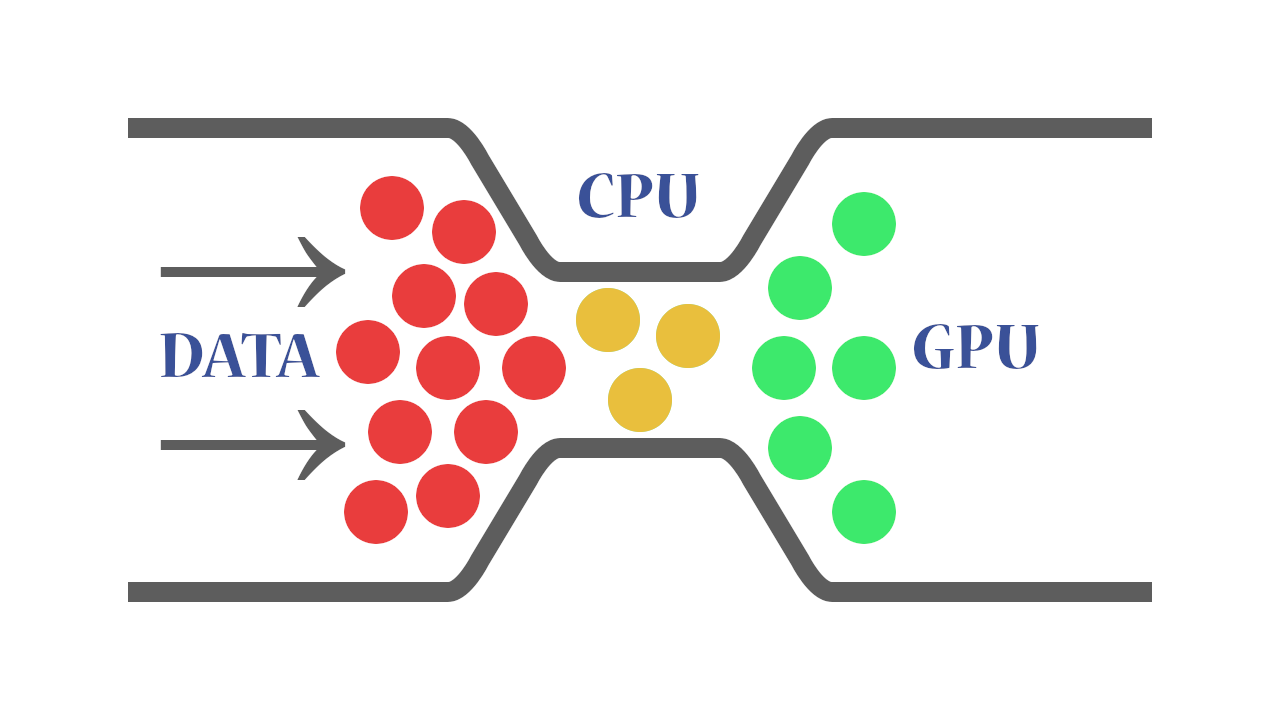
\includegraphics[width=\linewidth]{images/bottleneck.png}}
            \label{ris:bottleneck}
        \end{figure}
        
    \end{columns}
\end{frame}

%------------------------------------------------

\begin{frame}{Актуальность поставленной задачи}
    TensorFlow Lite (TF-Lite), PyTorch Mobile и CoreML — три наиболее популярных фреймворка для мобильного инференса — предоставляют абстрактные интерфейсы для работы с нейросетевыми моделями, но не обеспечивают тесной связки с текстурной памятью GPU и графическим пайплайном, основанным на OpenGL или Vulkan.
    \begin{columns}[c] % The "c" option specifies centered vertical alignment while the "t" option is used for top vertical alignment

        \column{.45\textwidth} % Right column and width
        \begin{figure}[h]
            \center{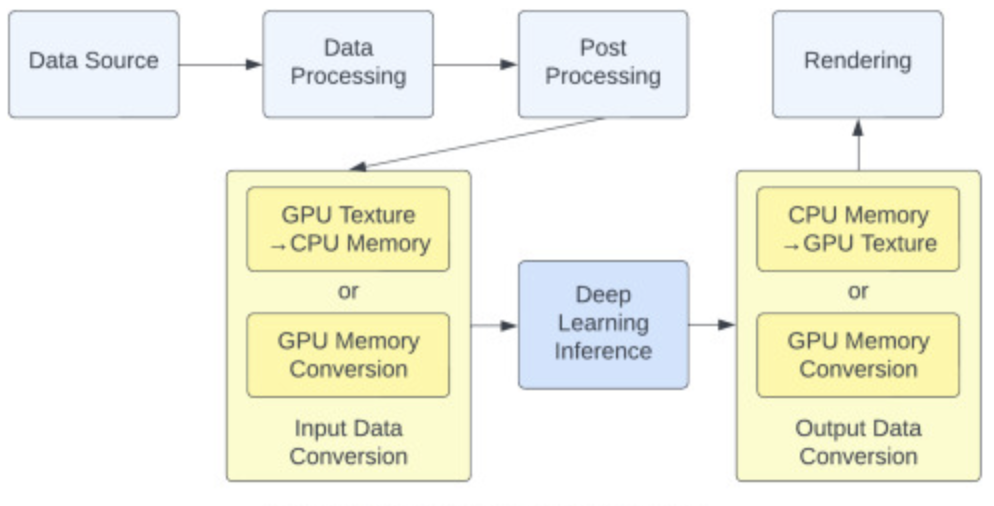
\includegraphics[width=\linewidth]{images/data.png}}
            \label{ris:ORTModelData}
        \end{figure}
        
        \column{.5\textwidth} % Left column and width
        \begin{itemize}
            \item Модели, содержащие редкие операторы, могут не поддерживаться GPU-бэкендом.
            \item Форматы Tensor или Mat, используемые в большинстве фреймворков, не совместимыми с текстурами OpenGL.
            \item Невозможность непосредственной передачи данных из шейдера в шейдер без выхода за пределы графического пайплайна затрудняет реализацию end-to-end решений.
        \end{itemize}

    \end{columns}
\end{frame}

%------------------------------------------------

\begin{frame}{Описание среды разработки}
    Для реализации GPU-only пайплайна в рамках задачи эффективного использования нейронных сетей на графических процессорах будут использоваться:
    
    \begin{block}{API доступа к GPU}
        OpenGL ES версии 3.20
    \end{block}

    \begin{block}{Модель}
        ESPCN\_2X\_16\_16\_4.h5
    \end{block}

    \begin{block}{Языки программирования, среда разработки и операционные системы}
        С++, Visual Studio и Windows, Android Studio и Android
    \end{block}
\end{frame}

%------------------------------------------------

\begin{frame}{Основные этапы конвейера}
    Разработанный пайплайн можно разделить на четыре основных этапа:
    \begin{columns}[c] % The "c" option specifies centered vertical alignment while the "t" option is used for top vertical alignment

        \column{.45\textwidth} % Left column and width
        \begin{figure}[h]
            \center{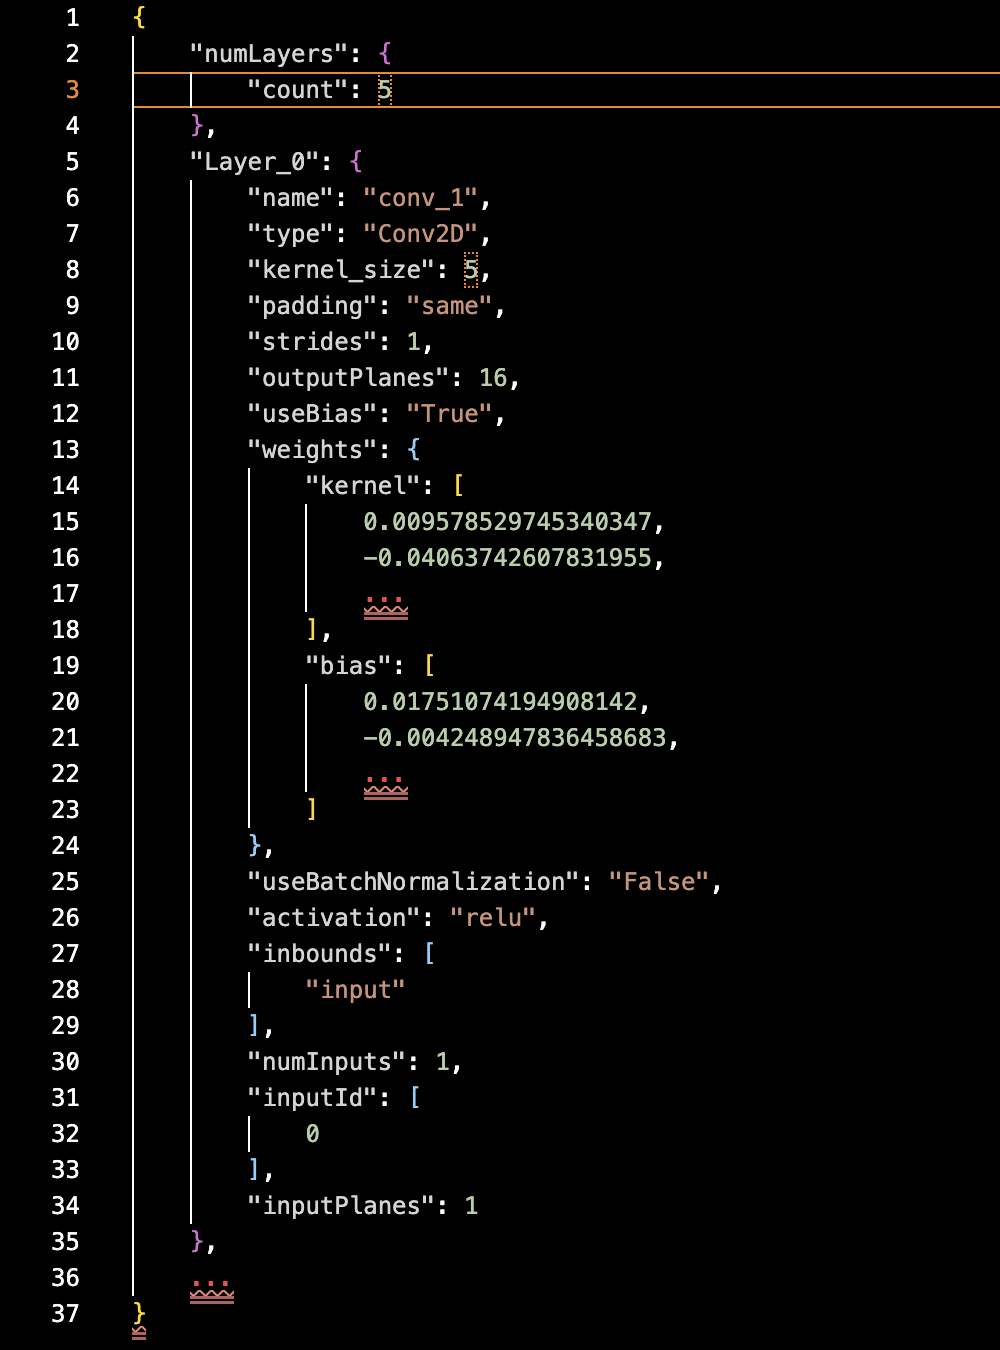
\includegraphics[width=0.7\linewidth]{images/json.png}}
            \label{ris:ORTModelData}
        \end{figure}

        \column{.5\textwidth} % Right column and width
        \begin{enumerate}
            \item Преобразование модели в удобный для работы формат — json файл;
            \item Загрузка модели и манипуляции с ней;
            \item Генерация вычислительного графа и необходимая предобработка;
            \item Выполнение соответствующих операторов для обработки модели.
        \end{enumerate}

    \end{columns}
\end{frame}

%------------------------------------------------

\begin{frame}{Архитектура фрагментных шейдеров для нейросетевых слоев}
    Для универсальности фрагментные шейдеры будут создаваться непосредственно после извлечения данных из файла модели, при этом будут использоваться шаблоны (для каждого слоя они уникальны), написанные заранее.
    
    Ниже приведена таблица, в которой перечислены слои модели ESPCN и соответствующие им количества render pass:

    \begin{table}[H]
        \begin{center}
            \begin{tabular}{|l|l|}
                \hline
                Модель ESPCN & Количество render pass \\
                \hline
                Layer 1: Conv2D output: $n \times n \times 16$ & Layer 1 output: 4 render passes \\
                \hline
                Layer 2: Conv2D output: $n \times n \times 16$ & Layer 2 output: 4 render passes \\
                \hline
                Layer 3: Conv2D output: $n \times n \times 4$ & Layer 3 output: 1 render pass \\
                \hline
                Layer 4: Subpixel output: $2n \times 2n \times 1$ & Layer 4 output: 1 render pass \\
                \hline
            \end{tabular}
        \end{center}
    \end{table}
\end{frame}

%------------------------------------------------

\begin{frame}{Реализация слоя Conv2D}
    \begin{columns}[] % The "c" option specifies centered vertical alignment while the "t" option is used for top vertical alignment

        \column{.5\textwidth} % Right column and width
        Главные аспекты шейдера:
        \begin{itemize}
            \item Поддерживаемые режимы pading: clamped, const, replicate, checkboard и remove\_zero.
            \item Три режима работы с весами: constants (загружаются на этапе создания шейдера), textures (передаются как текстуры) и buffers (передаются как буфферы).
            \item Реализована встроенная batch нормализация (если слой ее поддерживает).
            \item Присутствует режим MRT.
        \end{itemize}

        \column{.5\textwidth} % Left column and width
        \begin{figure}[h]
            \center{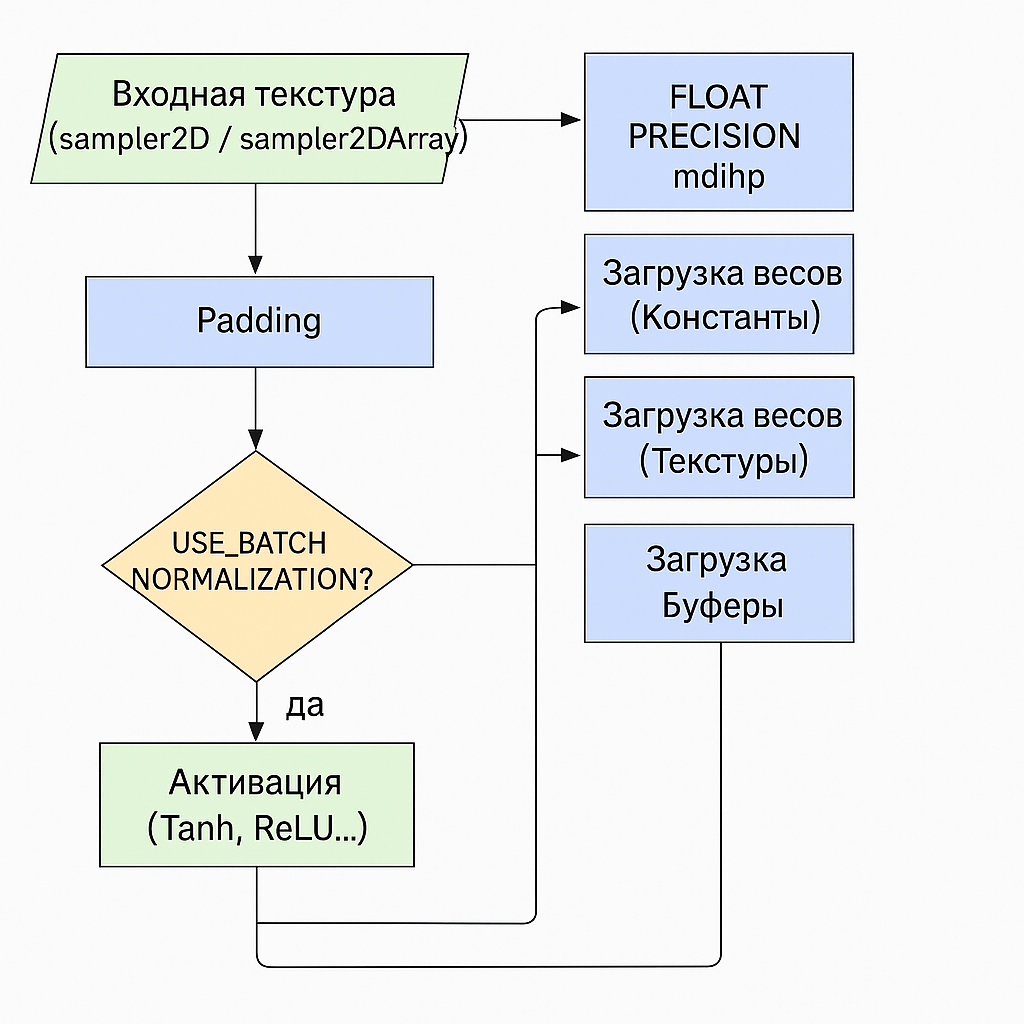
\includegraphics[width=\linewidth]{images/conv2d.png}}
            \label{ris:ORTModelData}
        \end{figure}
        
    \end{columns}
\end{frame}

%------------------------------------------------

\begin{frame}{Реализация слоя Activation}
    \begin{columns}[] % The "c" option specifies centered vertical alignment while the "t" option is used for top vertical alignment

        \column{.5\textwidth} % Left column and width
        \begin{figure}[h]
            \center{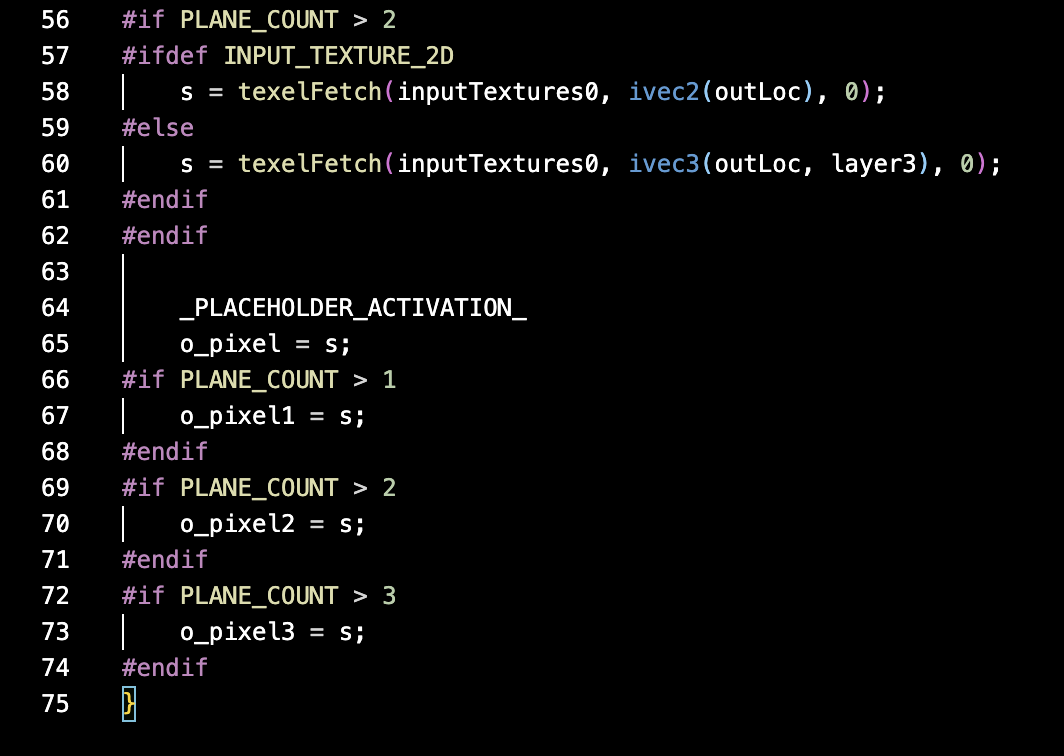
\includegraphics[width=\linewidth]{images/activation.png}}
            \label{ris:ORTModelData}
        \end{figure}

        \column{.5\textwidth} % Right column and width
        Реализованные функции активации:
        \begin{itemize}
            \item \textbf{ReLU:} s = max(s, vec4(0.0));
            \item \textbf{ReLU6:} s = clamp(s, vec4(0.0), vec4(6.0));
            \item \textbf{Tanh:} s = tanh(s);
            \item \textbf{Sigmoid:} s = vec4(1.0f) / (vec4(1.0f) + exp(-s));
            \item \textbf{LeakyReLU (с параметром alpha):}\\ s = max(s, (s * vec4(alpha)));
            \item \textbf{SiLU (Swish):}\\ s = s * vec4(1.0f) / (vec4(1.0f) + exp(-s));
        \end{itemize}
    \end{columns}
\end{frame}

%------------------------------------------------

\begin{frame}{Сравнительное тестирование реализованного пайплайна}
    \begin{figure}[h]
        \center{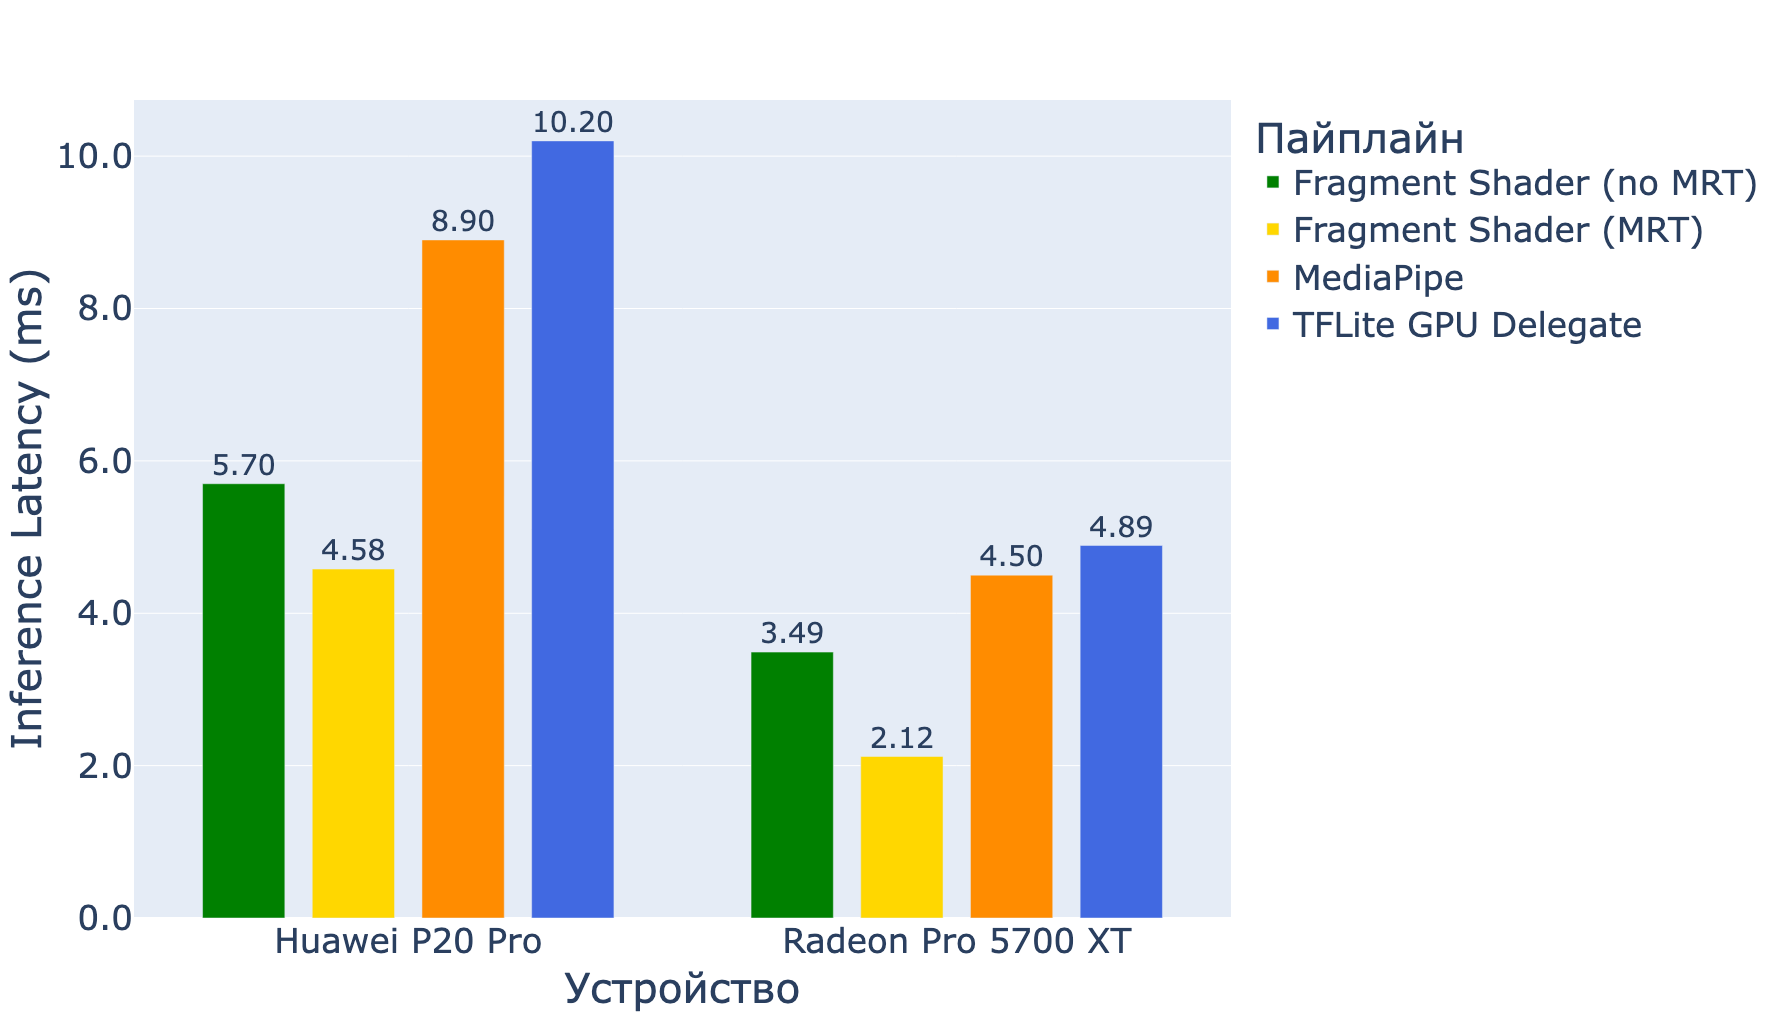
\includegraphics[width=0.8\linewidth]{images/graphic.png}}
        \label{ris:ORTModelData}
    \end{figure}
    
    % \begin{columns}[] % The "c" option specifies centered vertical alignment while the "t" option is used for top vertical alignment

    %     \column{.5\textwidth} % Left column and width
    %     \begin{itemize}
    %         \item Реализованный пайплайн тестировался на устройствах: Huawei P20 Pro на базе графического процессора ARM Mali-G72 MP12 и ноутбук с дискретной графикой AMD Radeon Pro 5700 XT.
    %         \item Сравнение происходило в рамках использования сторонних фреймворков MediaPipe и TFLite с GPU delegate.
    %     \end{itemize}
        
    %     \column{.5\textwidth} % Right column and width
    %     \begin{figure}[h]
    %         \center{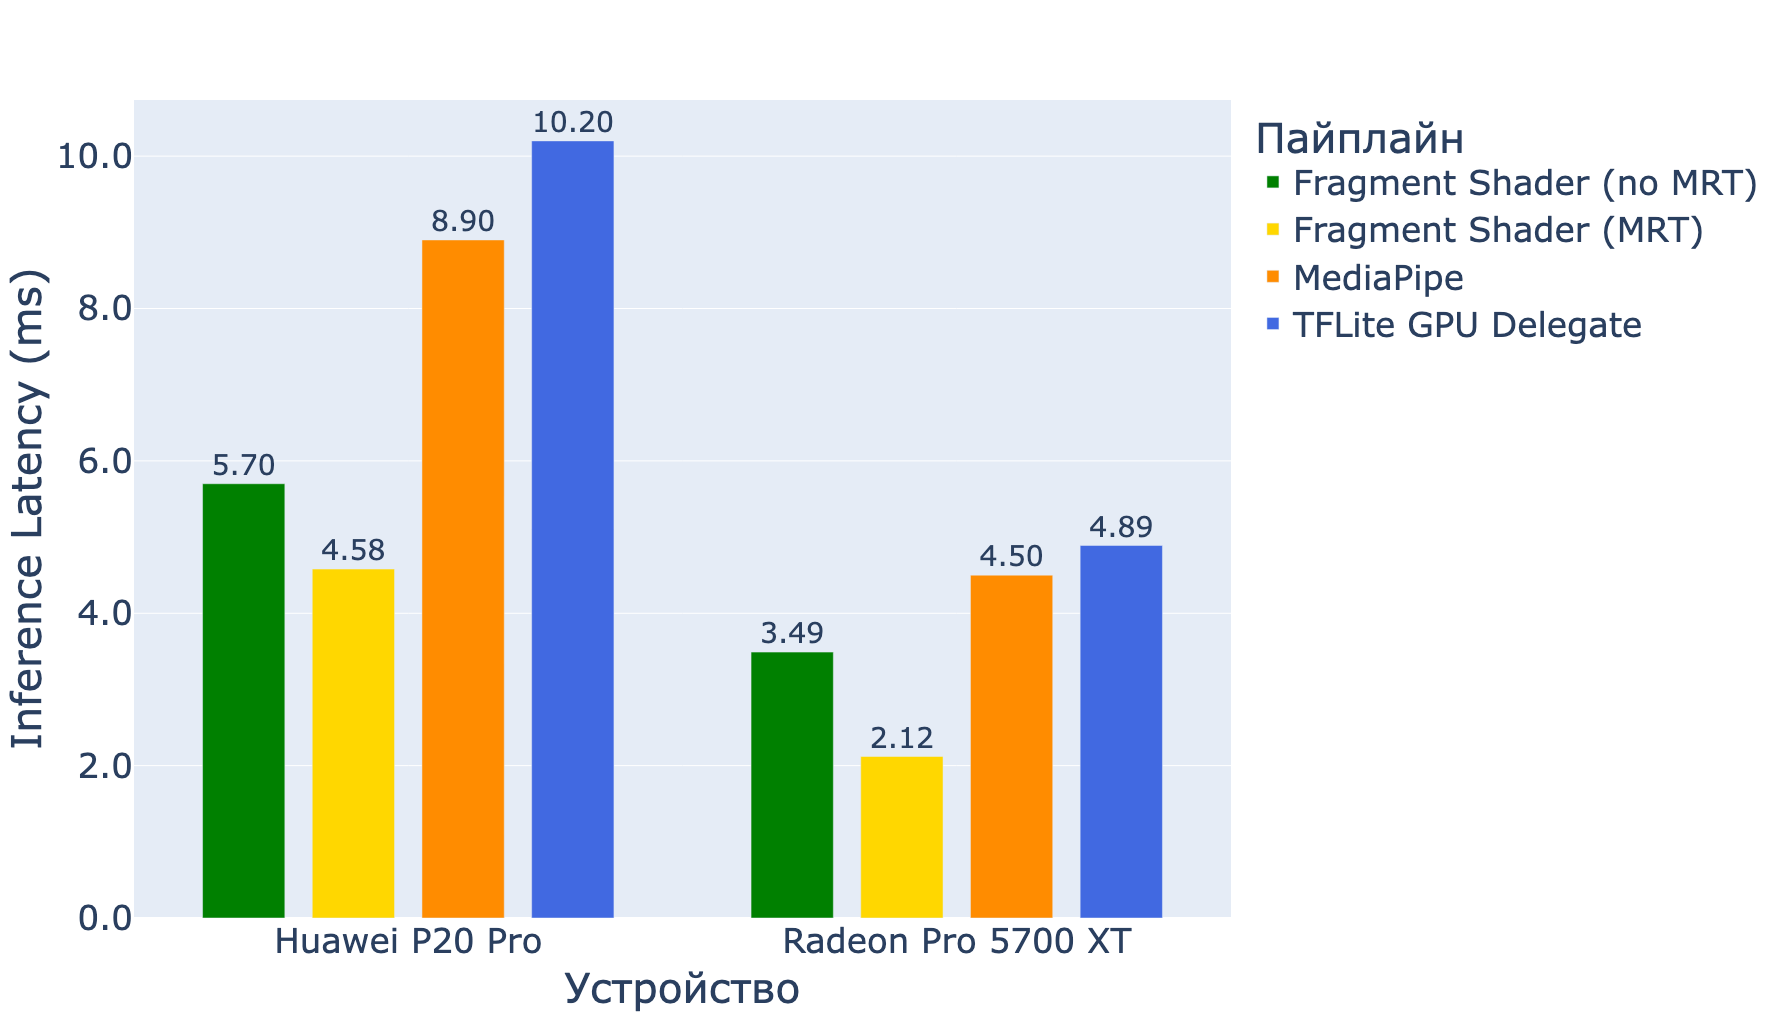
\includegraphics[width=\linewidth]{images/graphic.png}}
    %         \label{ris:ORTModelData}
    %     \end{figure}
    % \end{columns}
\end{frame}

%------------------------------------------------

\begin{frame}{Выводы}
    \begin{enumerate}
        \item Произведен анализ существующих реализаций GPU пайплайнов и их особенностей. Показано, что главном проблемой является отсутствие фреймворков с поддержкой аппаратных структур данных GPU для входа.
        \item Был реализован пайплайн на языке программирования С++, в основе которого лежит движок OpenGL.
        \item Разработана архитектура обработки данных на шейдерах (структура вершинного и фрагментного шейдера). Также реализованы шаблоны фрагментных шейдеров для слоев Conv2D, Activation и Subpixel.
        \item Проанализированы результаты сравнения построенного пайплайна с фреймворками MediaPipe и TFLite с GPU delegate. Среднее суммарное время обработки кадра нейросетью в реализованном пайплайне более, чем в 2 меньше, чем с помощью универсальных библиотек, что доказывает эффективность выбранного подхода.
    \end{enumerate}
\end{frame}

%-------------------------------------------------

\end{document}